\chapter{Discussion} \label{ch:Discussion}

This was a very ambitious project that aimed to deliver a cost-effective, and capable, impedance analyzer to hobbyists and small businesses. The initial focus on identifying a market gap provided a clear direction, ensuring that the project addressed the needs of the target group. The hardware development, particularly the sampling system, was a complete success. It effectively meets the core requirement of sampling the voltage and current signals, saving them in memory and allowing a microcontroller to process the samples and make the results available to the user, thus demonstrating that the fundamental design objectives were achieved. The sampling system is essentially developed as a full general purpose two channel data-logging system that could be used in many other systems.

However, not all aspects of the project met the intended specifications. Several software functionalities remain incomplete, such as much of the HMI. The HMI is intended to be build around a Nextion NX8048P070 Intelligent Series 7" touchscreen display development board \cite{NextionDisplay}. Although incomplete at the time of this report, the \textbf{work-in-progress} proposed interface is shown in Figure \ref{fig:7_3_3_NextionHMI}.

\begin{figure}[H] \centering 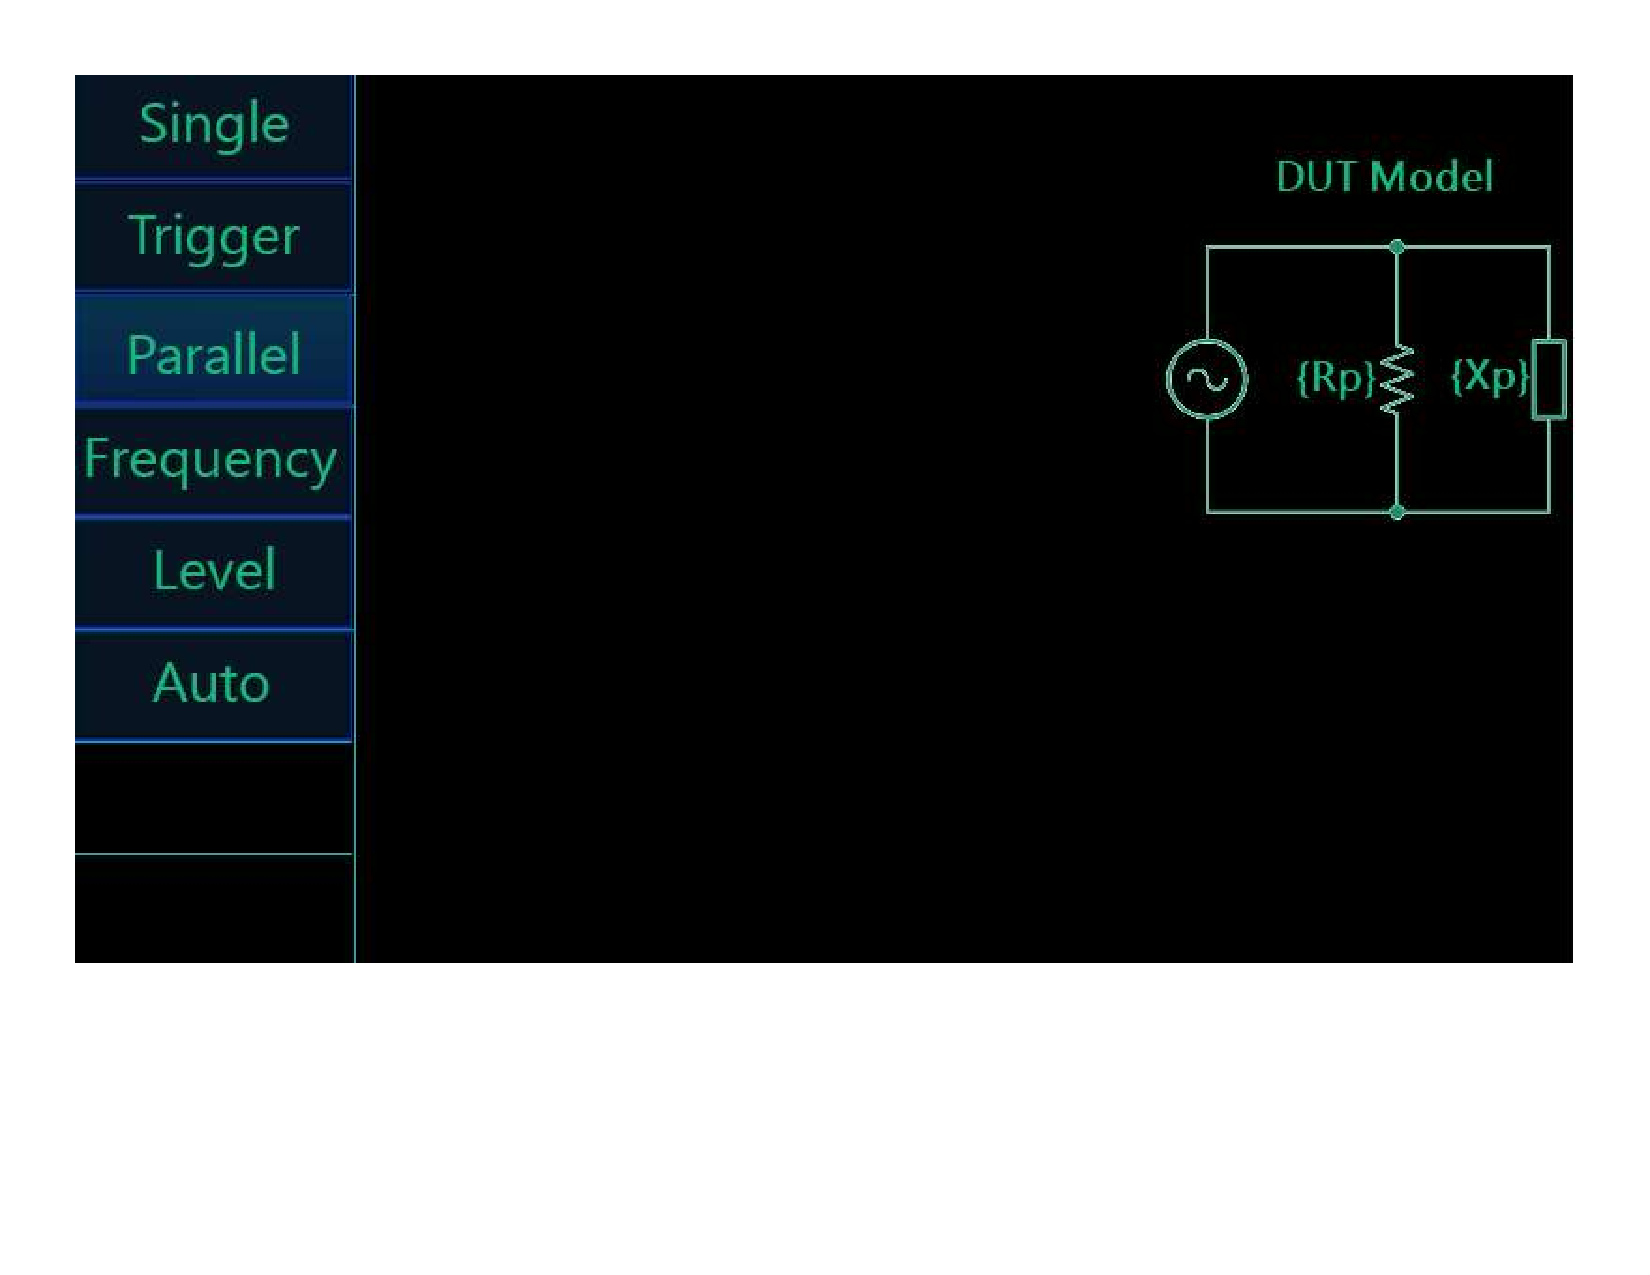
\includegraphics[clip, trim=0 150 0 0, width=0.65\textwidth]{Sections/7_SystemDesign/Figures/7_3_3_UIStatus.pdf} \caption{Current state of the HMI in the Nextion Editor. The UI includes buttons on the left side of the screen for setting various test parameters. The interface is currently in "single" measurement mode, indicated by the darkened "single" button. Pressing this button switches the interface to "sweep" mode, designed for generating plots as described earlier. The "parallel" model is selected, as shown by the corresponding highlighted button, which displays the parallel impedance model and measured parameters on the right side. The MCU detects whether the reactance is positive or negative and adjusts the Xp component to represent a capacitor or inductor accordingly. Final measurements of R, L, C, D, Q, and related parameters will be displayed in the center of the screen but are not yet implemented.} \label{fig:7_3_3_NextionHMI} \end{figure}

The Nextion platform simplifies integration using its proprietary display editor, which expedites the design process. The display communicates with the STM32 via UART, and basic data transfer has been successfully tested. However, a comprehensive data structure for display communication has not yet been implemented. One drawback of this platform is the time required to create graphical elements. Due to the absence of technical challenges in integrating this display, its development was assigned lower priority from the beginning of the project and remains incomplete. The lack of a useable HMI inhibits the Main Processor Module from having a fully functional main loop. While the Main Processor Module integrates all essential functions to interface with the Sample Control module, calibrate the instrument, enable auto-ranging features, and conduct spectral analysis. It is fully capable of initiating the sampling process, retrieving samples, analyzing them via spectral analysis, and calculating the impedance of the DUT as described in Section \refq{sec:ImpedanceAnalysis}.

As mentioned the HMI is not developed, but data from the impedance analyzer can be retrieved through a UART connection with the STM32, as shown in figure \refq{fig:7_3_3_CapMeasSerialPrint}.

\begin{figure}[H] \centering 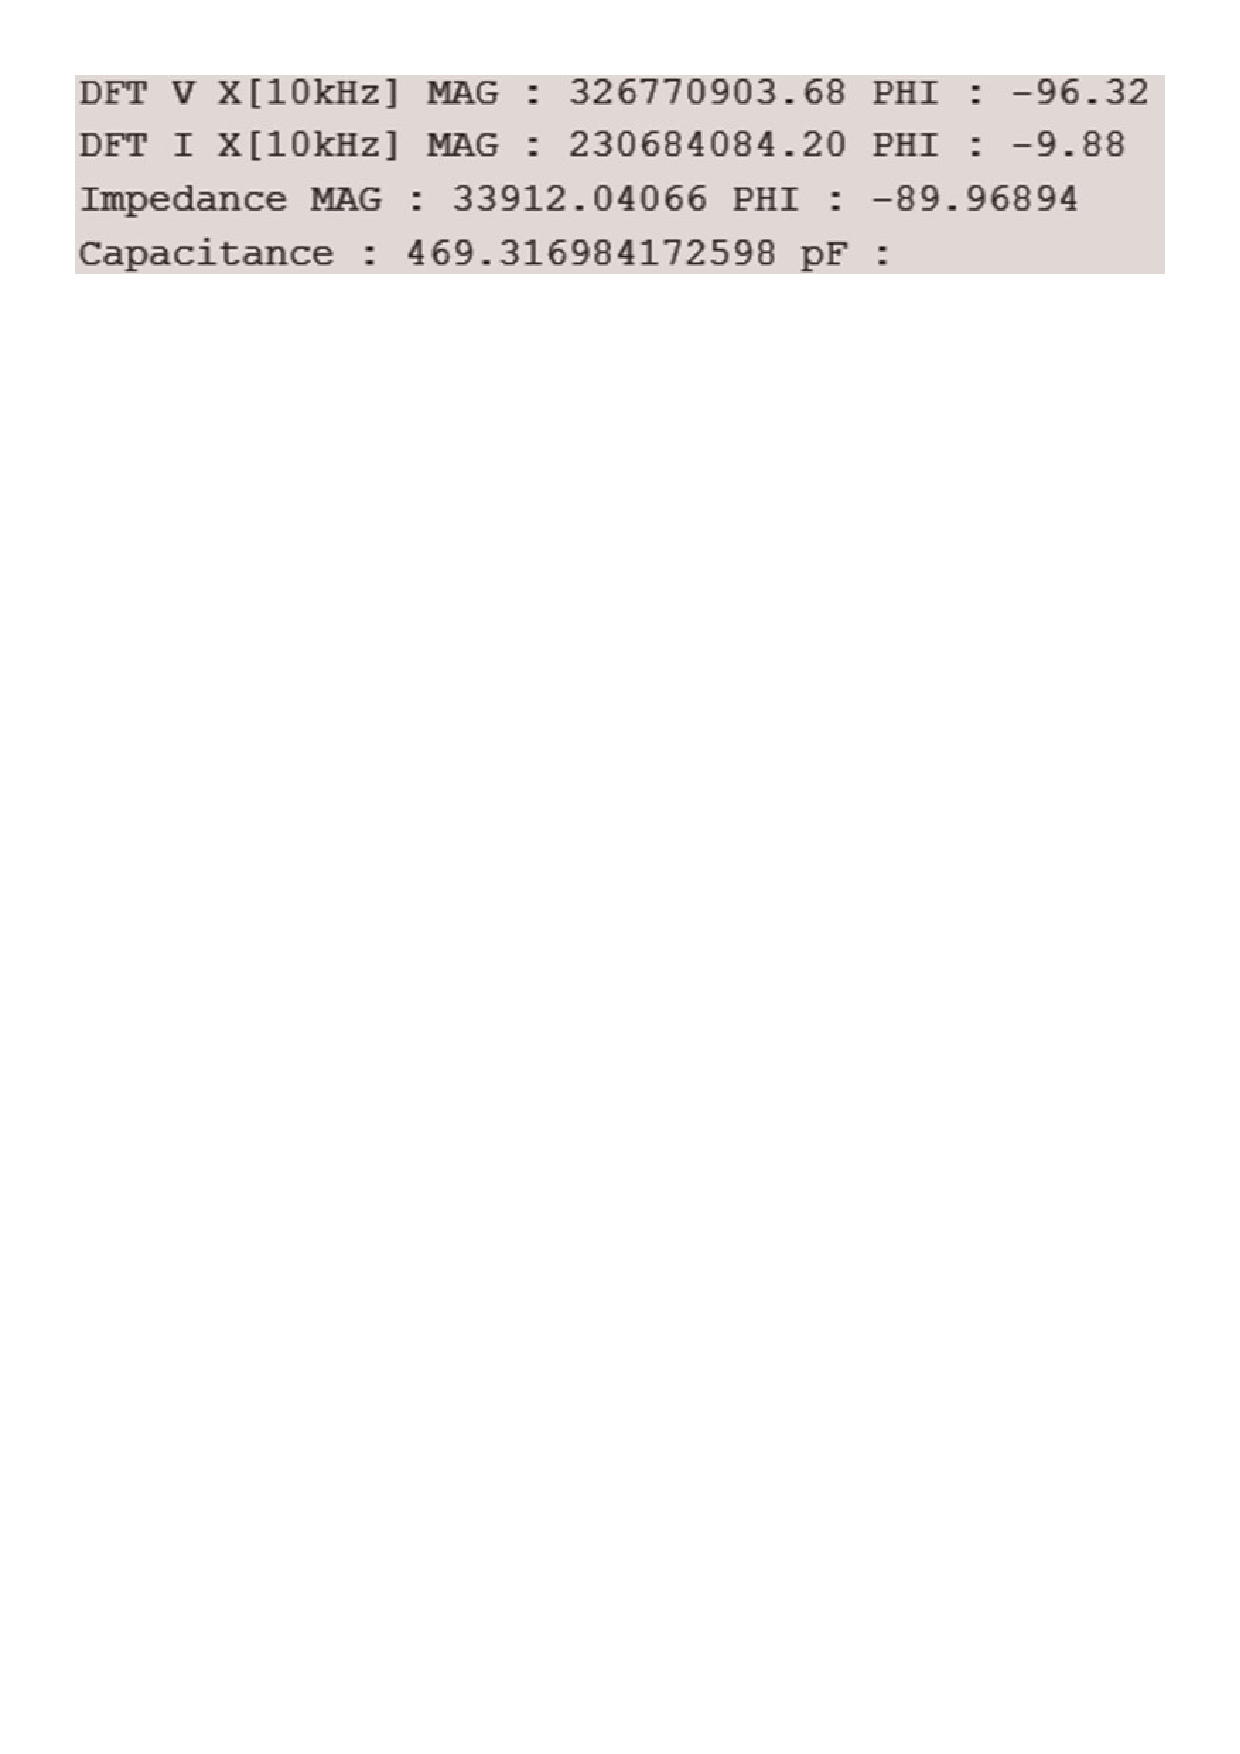
\includegraphics[clip, trim=0 700 0 0, width=0.65\textwidth]{Sections/7_SystemDesign/Figures/7_3_3_CapMeasuredSerialPrint.pdf} \caption{A DUT has been measured at \SIQ{10}{\kilo\hertz} by the impedance analyzer and the results are transmitted over a UART connection. Line 1-2 show the results from the DFT on the DUT voltage and currents. Line 3 shows the calculated impedance of the DUT in polar form and the magnitude and phase of the impedance is listed. Line 4 shows that the instrument has correctly identified the DUT as a capacitor with a value of about $470pF$. The DUT is a \SIQ{470}{\pico\farad} 1\% Mica capacitor.} \label{fig:7_3_3_CapMeasSerialPrint} \end{figure}

The instrument can take measurements of the DUT impedance as shown in figure \refq{fig:7_3_3_CapMeasSerialPrint} and display them to the user. Only the capacitance value of the DUT is shown, but it could also have listed the loss tangent, ESR or any other desired parameter as well.

In summary, the Main Processor Module includes all functionality required for the instrument to operate. However, the absence of finalized functions to display results to the user remains a limitation at this stage and a polished main() loop has not been developed.

From a more technical standpoint the project does not manage to pass all of the set requirements. Many of these are software functions that could be developed with time, they are not technically challenging to develop, just time consuming. It is not possible to verify the accuracy due to the lack of available reference capacitors, inductors, resistors and other test equipment. The test conducted indicates good accuracy, especially at low frequencies, at and below \SIQ{10}{\kilo\hertz}, at frequencies above this range the phase error drastically increases. The large phase error at these frequencies is expected to be caused by an incomplete open/short model for the fully differential output. 

The analog front-end is designed for a \SIQ{1}{\mega\hertz} bandwidth. The means of sampling these frequencies where originally intended to be done with a sub-sampling scheme. This however was never implemented and as a result the system has not been tested above \SIQ{300}{\kilo\hertz}.

A major focal point of this project has been to keep the costs at a minimum, a roughly estimated production cost of the developed system can be seen in appendix \refq{App:A_CostOverview}. The production cost of the proposed system is at a similar price-point as the Keysight handheld U1733C whilst having features typically seen on more advanced models such as the R\&S LCX-200.


